\subsubsection{Valori dell'indice di Gulpease}

Per ogni documento stilato è stato calcolato l'indice di Gulpease\glo{}. I valori sono dati dalla seguente tabella ed il rispettivo grafico con valore sufficiente >40 e valore ottimo >80.

\hphantom{}
\tabulinesep = 2mm % padding
\taburowcolors [1] 2{pari .. dispari} % colori delle righe

\begin{longtabu} to \textwidth {| X[0.2,c m]  | X[0.1,c m] | X[0.1,c m]| X[0.1,c m] | X[0.1,c m] |}
\hline
\rowcolor{header}
\textbf{Data del calcolo} &  
\textbf{Norme di Progetto} & 
\textbf{Analisi dei Requisiti} & 
\textbf{Piano di Qualifica} & 
\textbf{Piano di Progetto} \\
\hline

\multirow[c]{2}{*}{2020-12-03} & v0.1.0 & v0.2.4 & v0.2.1 & v0.1.0 \\
\cline{2-5} 
& 65 & 61 & 80 & 91 \\ 
\hline
\multirow[c]{2}{*}{2021-01-10} & v1.0.0 & v1.0.0 & v1.0.0 & v1.0.0 \\ 
\cline{2-5} 
 & 68 & 69 & 70 & 79 \\ 
\hline
\multirow[c]{2}{*}{2021-02-05}  & v1.0.1 & v1.0.5 & v1.0.2 & v1.0.2 \\ 
\cline{2-5} 
 & 75 & 74 & 64 & 83 \\ 
\hline
\multirow[c]{2}{*}{2021-02-20}  & v1.1.3 & v1.1.0 & v1.1.2 & v1.0.3 \\ 
\cline{2-5} 
 & 82 & 68 & 72 & 69 \\ 
\hline
\multirow[c]{2}{*}{2021-03-09} & v2.0.0 & v2.0.0 & v2.0.0 & v2.0.0 \\ 
\cline{2-5} 
 & 74 & 70 & 70 & 74 \\ 
\hline
\multirow[c]{2}{*}{2021-03-26}  & v2.0.2 & v2.1.0 & v2.0.1 & v2.0.3 \\ 
\cline{2-5} 
 & 73 & 69 & 70 & 73 \\ 
\hline
\multirow[c]{2}{*}{2021-03-4}  & v2.2.0 & v2.1.3 & v2.2.1 & v2.2.3 \\ 
\cline{2-5} 
 & 70 & 65 & 71 & 70 \\ 
\hline
\multirow[c]{2}{*}{2021-04-20}  & v3.0.0 & v3.0.0 & v3.0.0 & v3.0.0 \\ 
\cline{2-5} 
 & 68 & 64 & 72 & 68 \\ 
\hline
\end{longtabu}


\begin{figure}[H]
    \centering
    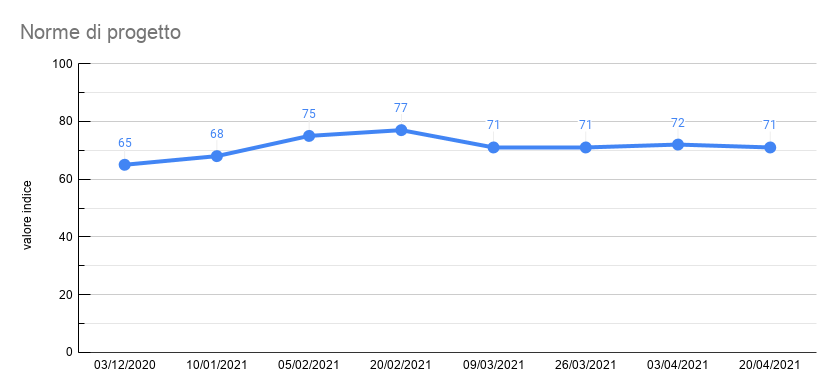
\includegraphics[width=13 cm]{source/sections/images/IdG_NdP.png}
    \caption{Indice di Gulpease - Norme di Progetto}
\end{figure}

\begin{figure}[H]
    \centering
    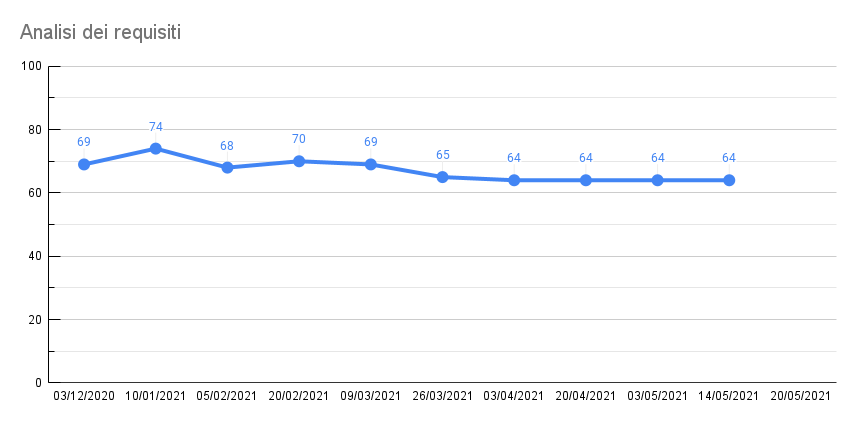
\includegraphics[width=13 cm]{source/sections/images/IdG_AR.png}
    \caption{Indice di Gulpease - Analisi dei Requisiti}
\end{figure}
\begin{figure}[H]
    \centering
    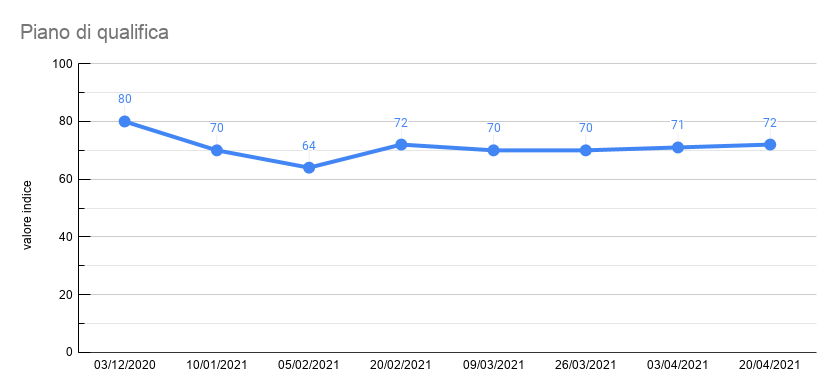
\includegraphics[width=13 cm]{source/sections/images/IdG_PdQ.png}
    \caption{Indice di Gulpease - Piano di Qualifica}
\end{figure}
\begin{figure}[H]
    \centering
    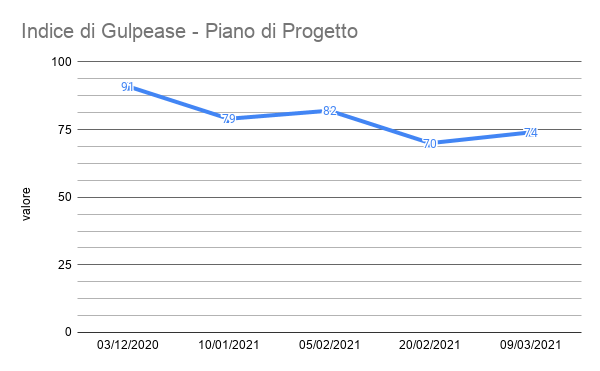
\includegraphics[width=13 cm]{source/sections/images/IdG_PdP.png}
    \caption{Indice di Gulpease - Piano di Progetto}
\end{figure}

\subsubsection{Errori ortografici}

Per quanto riguarda gli errori ortografici, oltre alla revisione fatta dai membri del gruppo, si è utilizzato anche lo spellchecker di Overleaf.

\newpage
\subsubsection{Percentuale di metriche soddisfatte}
    Per le metriche: Percentuale dei requisiti soddisfatti, complessità ciclomatica, sfin e sfout, alle quali sono stati determinati valori sufficienti e ottimi per ogni unità di calcolo,
    verranno considerate ottime se la maggior parte delle unità presenteranno valori ottimi. L'equivalente
    sarà considerato per i valori sufficienti e insufficienti. 


    \begin{longtabu} to \textwidth {| X[0.2,c m] | X[0.1,c m] | X[0.1,c m] |}
        \hline
        \rowcolor{header}
        \textbf{Metrica} &
        \textbf{Valore} &
        \textbf{Esito}\\
        \hline
        \hyperlink{subsubsection.5.1.1}{percentuale requisiti soddisfatti}& 74\% & insufficiente \\ 
        \hline
        \hyperlink{subsubsection.5.1.2}{Earned Value} & 5935 & ottimo  \\ 
        \hline
        \hyperlink{subsubsection.5.1.2}{Planned Value} & 5935 & ottimo  \\
        \hline
        \hyperlink{subsubsection.5.1.2}{Actual cost} & 5935 & ottimo  \\
        \hline
        \hyperlink{subsubsection.5.1.2}{Schedule variance Value} & 0 & ottimo  \\
        \hline
        \hyperlink{subsubsection.5.1.2}{Cost variance Value} & 0 & ottimo  \\
        \hline
        \hyperlink{subsubsection.5.2.1}{Errori ortografici} & 0 & ottimo  \\
        \hline
        \hyperlink{subsubsection.5.2.4}{Code coverage} & 12\% & insufficiente \\
        \hline
        \hyperlink{subsubsection.5.2.5}{Numero di test superati} & 57,6\% & insufficiente \\
        \hline
        \hyperlink{subsubsection.5.3.1}{Numero di click} & 2 & ottimo \\
        \hline
        \hyperlink{subsubsection.5.3.2}{Site depth} & 1 & ottimo \\
        \hline
        \hyperlink{subsubsection.5.3.3}Response time & 54,8 & ottimo \\
        \hline
        \hyperlink{subsubsection.5.3.4}{Complessità ciclomatica} & 99\% & ottimo \\
        \hline
        \hyperlink{subsubsection.5.3.5}{Facilità di comprensione} & 0.026 & insufficiente \\
        \hline
        \hyperlink{subsubsection.5.3.6}{sfin} & 59\% & Sufficiente \\
        \hline
        \hyperlink{subsubsection.5.3.6}{sfout} & 72\% & sufficiente \\
        \hline
        
        \end{longtabu}

        \begin{figure}[H]
            \centering
            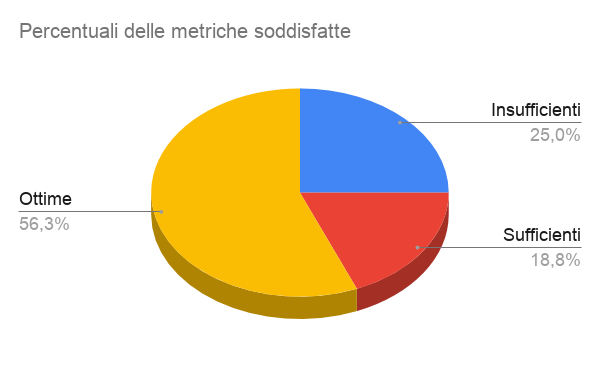
\includegraphics[width=14 cm]{source/sections/images/percentuale-metriche-soddisfatte.png}
            \caption{Grafico delle metriche soddisfatte}
        \end{figure}

\subsubsection{Code coverage}
    in questa fase del progetto didattico non si è data piena precedenza al numero di righe testate. E' stata comunque
    iniziata parzialmente una parte di testing. In seguito i valori del Code coverage calcolati dal 20 Marzo al 20 Aprile
    \begin{figure}[H]
        \centering
        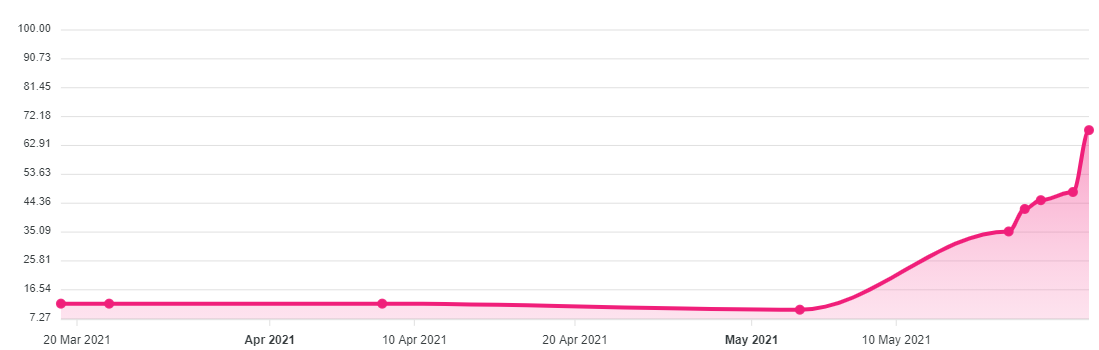
\includegraphics[width=16 cm]{source/sections/images/CodeCoverage.png}
        \caption{Grafico dei valori del Code coverage - GitHub}
    \end{figure}


\subsubsection{Numero di test superati}

    \begin{figure}[H]
        \centering
        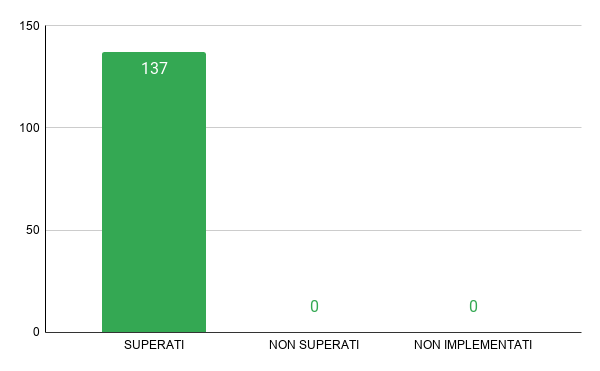
\includegraphics[width=10 cm]{source/sections/images/num-test.png}
        \caption{Grafico numero di test}
    \end{figure}

    \begin{figure}[H]
        \centering
        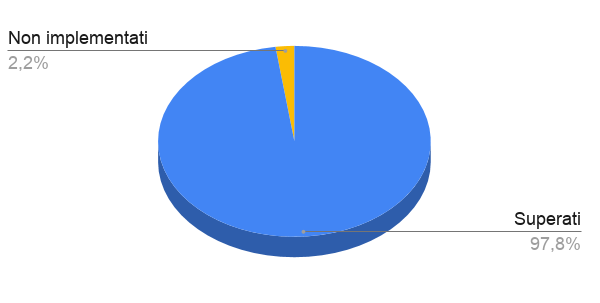
\includegraphics[width=10 cm]{source/sections/images/torta-test.png}
        \caption{Grafico della percentuale dei test}
    \end{figure}
